\documentclass[tikz,crop,convert={density=300,outext=.png},border=0.3cm,width=18cm,height=3cm]{standalone}
%\documentclass[tikz,border=0.3cm]{standalone}
\usepackage[left=2.2cm,right=2.2cm,top=2.5cm,bottom=2.0cm,a4paper]{geometry}
\usepackage{pgfplots}
\usepackage{amsmath}
\usetikzlibrary{arrows.meta}
\usepackage{physics}
\pgfplotsset{compat=newest,
    %width=6cm,
    %height=3cm,
    scale only axis=true,
    max space between ticks=25pt,
    try min ticks=5,
    every axis/.style={
        axis y line=middle,
        axis x line=middle,
        axis line style={thick,->,>=latex, shorten >=-.3cm}
    },
      every axis plot/.append style={thick},
    tick style={black, thick},
}
\tikzset{
    semithick/.style={line width=0.8pt},
}
\usepgfplotslibrary{groupplots}
\usepgfplotslibrary{dateplot}
\usetikzlibrary{positioning}
%\pgfplotsset{compat=1.17}

\begin{document}
\begin{tikzpicture}
\node[inner sep=0pt] (mixed) at (-4,0)
{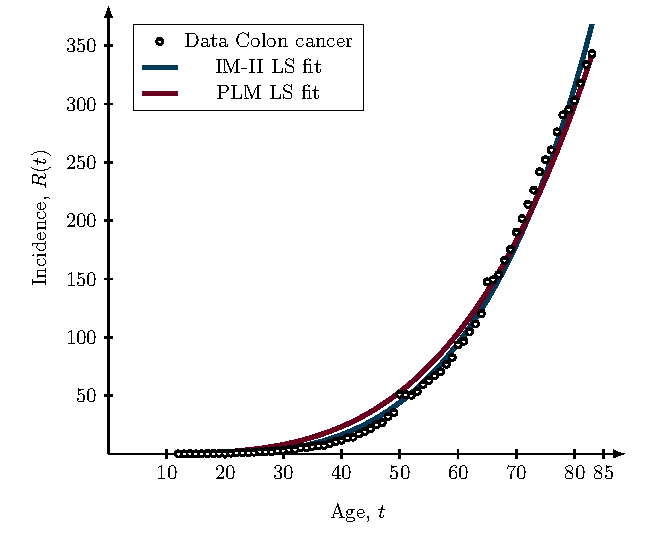
\includegraphics[width=0.5\textwidth]{{./colon/colon_LS.pdf}}};
\node[inner sep=0pt] (power_law) at (4,0)
{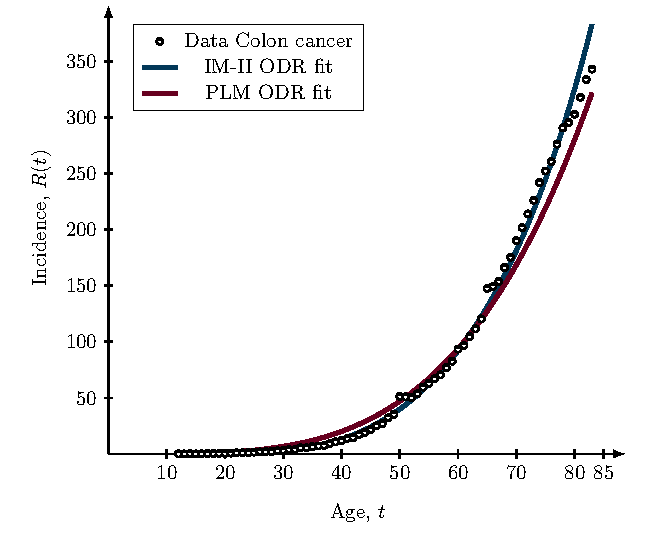
\includegraphics[width=0.5\textwidth]{{./colon/colon_ODR.pdf}}};
% \node[inner sep=0pt] (exponential) at (0,-8)
    %{\includegraphics[height=0.33\textheight]{{./CML/CML.pdf}}};

\node (b) at (0.25,4) {\large (\textbf{B})};
\node[left=7cm of b] (a) {\large (\textbf{A})};
%\node[below=7cm of b] (c) {\large (\textbf{C})};
%\draw (-2.35,-4) -- (-2.35,4);
\end{tikzpicture}

\end{document}
